In this section, we will discuss the benefits of high-order finite element operators implemented in a matrix free fashion.
First we will discuss how matrix-free implementation better agrees with system balance on modern HPC hardware.
Then we will highlight the spectral convergence properties of high-order methods.

% -- Storage and FLOPs --------------------------------------------------------
\subsection{Storage and FLOPs}

To demonstrate the performance benefits of high-order finite elements implemented in a matrix-free fashion, we consider the specific case of the scalar screened Poisson equation, $\nabla^2 u - \alpha^2 u = f$.
We consider the approximate number of bytes required for storage and FLOPs required to apply a matrix-vector product representing a high-order finite element operator corresponding to the Galerkin system for the screened Poisson equation.

With a sparse matrix representation, application of the finite element operator for a single element requires $\mathcal{O} \left( p^6 \right)$ matrix entries and $\mathcal{O} \left( p^6 \right)$ floating point operations.
In contrast, application of the matrix-free operator for a single tensor product element requires $\mathcal{O} \left( p^3 \right)$ floating point values and $\mathcal{O} \left( p^{d + 1} \right)$ floating point operations.
When multiple components in the PDE use the same finite element bases, the coefficients in this complexity analysis further favor matrix-free operator implementations.

\begin{figure}[h!]
\begin{subfigure}{.495\textwidth}
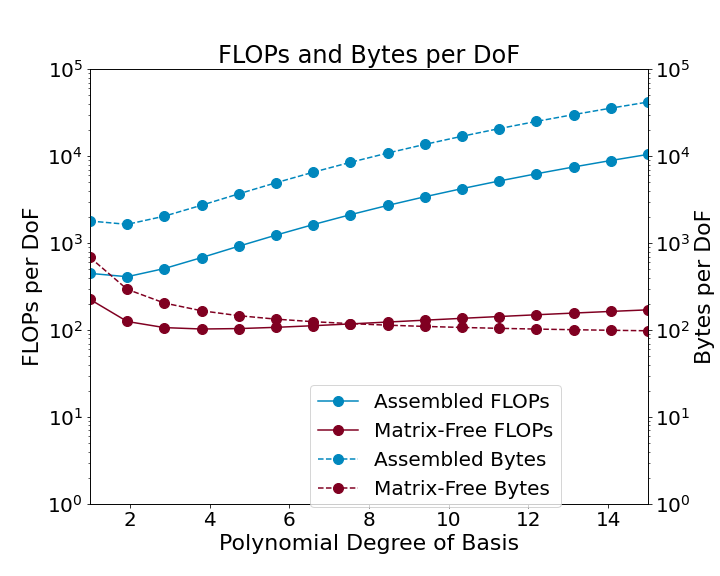
\includegraphics[width=.99\linewidth]{img/assembledVsMatrixFree}
\caption{FLOPs and Bytes per DoF}
\end{subfigure}
\begin{subfigure}{.495\textwidth}
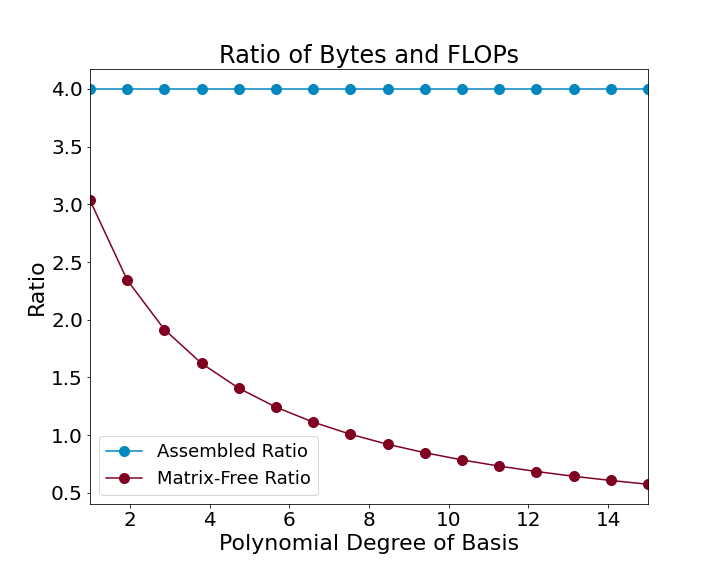
\includegraphics[width=.99\linewidth]{img/assembledVsMatrixFreeBalance}
\caption{Ratio of Bytes to FLOPs}
\end{subfigure}
\caption{Performance per DoF}
\label{fig:assembledvsmatrixfree}
\end{figure}

As seen in Figure \ref{fig:assembledvsmatrixfree}, the balance between bandwidth and FLOPs for matrix-free implementations with tensor product finite elements more closely agrees with current HPC hardware capabilities shown in Figure \ref{fig:peakratio}.
Matrix-free finite element operator implementations allow for greater arithmetic intensity at high-order, which allows these operators to achieve performance that is closer to the peak performance for this hardware.

It is important to note that generation of high quality hexahedral meshes for tensor product finite elements is a time intensive process when compared to the generation of simplex meshes.
However, it is possible to generate meshes comprised predominately of high quality hexahedral elements with initial refinement of a simplex mesh without the costly process of fully converting a simplex mesh into hexahedral elements.
Thus, the performance benefits of high-order matrix-free finite elements can be realized without the substantial additional effort required to generate a mesh exclusively composed of high quality hexahedral elements.

% -- Spectral Accuracy --------------------------------------------------------
\subsection{Spectral Accuracy}
